\documentclass[tikz,border=9pt,12pt]{standalone}
\usepackage{amsmath,amssymb}
\usetikzlibrary{arrows.meta,calc}
\tikzset{every node/.style={text=black,font=\normalsize},axis/.style={-{Stealth[length=2mm]},black!65,thin},vec/.style={-{Stealth[length=2.8mm]},line width=1.3pt,blue!70!black},lab/.style={fill=white,inner sep=2pt}}
\begin{document}
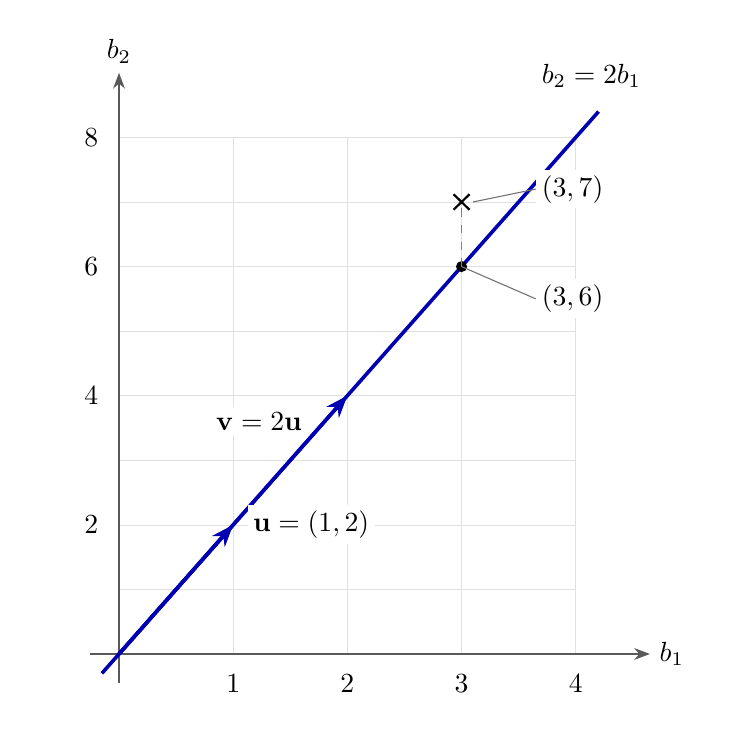
\begin{tikzpicture}[x=1.45cm,y=.82cm]
\path[use as bounding box] (-.8,-1.05) rectangle (5.2,9.7);
\draw[step=1,black!12,very thin] (0,0) grid (4,8);
\draw[axis] (-.25,0)--(4.65,0) node[right] {$b_1$};
\draw[axis] (0,-.45)--(0,9) node[above] {$b_2$};
\foreach \t in {1,2,3,4} {\node[below=4pt] at (\t,0) {$\t$};}
\foreach \t in {2,4,6,8} {\node[left=4pt] at (0,\t) {$\t$};}
\draw[blue!70!black,line width=1.3pt] (-.15,-.3)--(4.2,8.4);
\node[lab,right] at (3.65,8.95) {$b_2=2b_1$};
\draw[vec] (0,0)--(2,4);
\node[lab,right=5pt] at (1,2) {$\mathbf u=(1,2)$};
\draw[vec] (0,0)--(1,2);
\node[lab,left=6pt] at (1.8,3.6) {$\mathbf v=2\mathbf u$};
\fill (3,6) circle (2pt);
\draw[black!55,thin] (3,6)--(3.65,5.5);
\node[lab,right] at (3.65,5.5) {$(3,6)$};
\draw[black,thick] (2.93,6.88)--(3.07,7.12) (2.93,7.12)--(3.07,6.88);
\draw[black!55,thin] (3.1,7)--(3.65,7.2);
\node[lab,right] at (3.65,7.2) {$(3,7)$};
\draw[black!50,dashed] (3,6)--(3,7);
\end{tikzpicture}
\end{document}
